\documentclass{thesis}


% 定理类环境宏包
\usepackage{amsthm}

% 插图
\usepackage{graphicx}

% 三线表
\usepackage{booktabs}

% 表注
\usepackage{threeparttable}

% 跨页表格
\usepackage{longtable}

% SI 量和单位
\usepackage{siunitx}

% 配置图片的默认目录
\graphicspath{{figures/}}

% 数学命令
\makeatletter

\makeatother
\newcommand\eu{{\symup{e}}}
\newcommand\iu{{\symup{i}}}

\usepackage[backend=bibtex]{biblatex}

% hyperref 宏包在最后调用
\usepackage{hyperref}

\title{南京农业大学本科学位论文}
{ \LaTeX 模板示例文档}{A Sample Document for \LaTeX-based NJAU Thesis Template}
\college{公共管理学院}
\major{数学与应用数学}
\class{数学 114}
\studentnumber{114514191}
\author{ \LaTeX }
\advisor{ \LaTeX }
\advisortitle{副教授}

\begin{document}

\makecover

\copyrightpage

\pagenumbering{Roman}%中英文摘要要求使用罗马数字
\begin{cnabstract}
    摘要分中文和英文两种,中文在前,英文在后,博士论文中文摘要一般 800~1500 个汉字,硕士论文中文摘要一般 500~1000 个汉字。
    英文摘要的篇幅参照中文摘要。

    关键词另起一行并隔行排列于摘要下方,左顶格,中文关键词间空一字或用分号“,”隔开,英文关键词之间用逗号“,”或分号“;”隔开。

    中文摘要是论文内容的总结概括,应简要说明论文的研究目的、基本研究内容、研究方法或过程、结果和结论,突出论文的创新之处。
    摘要应具有独立性和自明性,即不用阅读全文,就能获得论文必要的信息。
    摘要中不宜使用公式、图表,不引用文献。

    中文关键词是为了文献标引工作从论文中选取出来用以表示全文主题内容信息的单词和术语,一般 3~8 个词,要求能够准确概括论文的核心内容。
    \begin{cnkeywords}
        LaTeX;摘要
    \end{cnkeywords}
\end{cnabstract}

\begin{enabstract}
    This is a sample document of NJAU thesis \LaTeX{} template for bachelor majoring in natural science subjects.

    It is worth noting that this thesis \LaTeX{} template has not been reviewed and authorized by the relevant departments of the university, please be sure to exercise discretion before using it.

    Users need to know that there are potential thesis formatting review issues.
    \begin{enkeywords}
        LaTeX; ABSTRACT
    \end{enkeywords}
\end{enabstract}
\pagenumbering{arabic}

\tableofcontents

\mainpart

\section{文献综述}
\fontsize{12pt}{0pt}
\par \LaTeX 是由Leslie Lamport自主研发的一款全新\TeX 格式。
故事发生在一个被称作「地球」的真实世界,在这里,你将扮演一位名为「创作者」的神秘角色,导引排版公式之力,在自由的编辑中邂逅性格各异、能力独特的同伴们,和他们一起,利用强大的排版引擎和丰富的宏包库,自由地构建你的学术论文
——同时,逐步发掘「排版」的真相。

\section{数学}
\subsection{数字和单位}

\begin{itemize}
    \item \unit{\mu}
    \item \unit{\eta}
    \item \unit{\lambda}
    \item \unit{\xi}
\end{itemize}

\subsection{数学符号和公式}

\begin{equation}
    \vec{F}=m\frac{d\vec{v}}{dt}+\vec{v}\frac{dm}{dt}
\end{equation}

\subsection{证明}
\begin{proposition}
    Suppose $f$ is integrable on $\mathbb{R}^d$. Then for every $\epsilon > 0$:
    \begin{enumerate}
        \renewcommand{\theenumi}{\roman{enumi}}
        \item There exists a set of finite measure $B$ (a ball, for example) such
              that
              \begin{equation}
                  \int_{B^c} |f| < \epsilon.
              \end{equation}
        \item There is a $\delta > 0$ such that
              \begin{equation}
                  \int_E |f| < \epsilon \qquad \text{whenever } m(E) < \delta.
              \end{equation}
    \end{enumerate}
\end{proposition}
\begin{theorem}
    Suppose $\{f_n\}$ is a sequence of measurable functions such that
    $f_n(x) \to f(x)$ a.e. $x$, as $n$ tends to infinity.
    If $|f_n(x)| \le g(x)$, where $g$ is integrable, then
    \begin{equation}
        \int |f_n - f| \to 0 \qquad \text{as } n \to \infty,
    \end{equation}
    and consequently
    \begin{equation}
        \int f_n \to \int f \qquad \text{as } n \to \infty.
    \end{equation}
\end{theorem}

\section{图片与引用}
Front identification at the surface is important for defining WRs and
FRs. Generally, front identification is based on the gradient of ground or
low-level meteorological elements. The inclining feature of fronts together with the hilly terrain in South China make objective front
identification quite difficult. Therefore, in this paper, the locations of
fronts are analyzed by forecasters who subjectively locate fronts using a
combination of temperature and wind observations in the surface and
925-hPa layers. Specifically, if a front is strong (clear) enough in the
surface analyses, we locate the fronts based on the hourly surface observations (mainly by significant temperature gradients). Otherwise, we
determine the fronts mainly based on the 925-hPa directional wind
shear (significant difference in wind direction) and temperature gradients\cite{WU2020104693}
\begin{figure}[htbp]
	\centering
	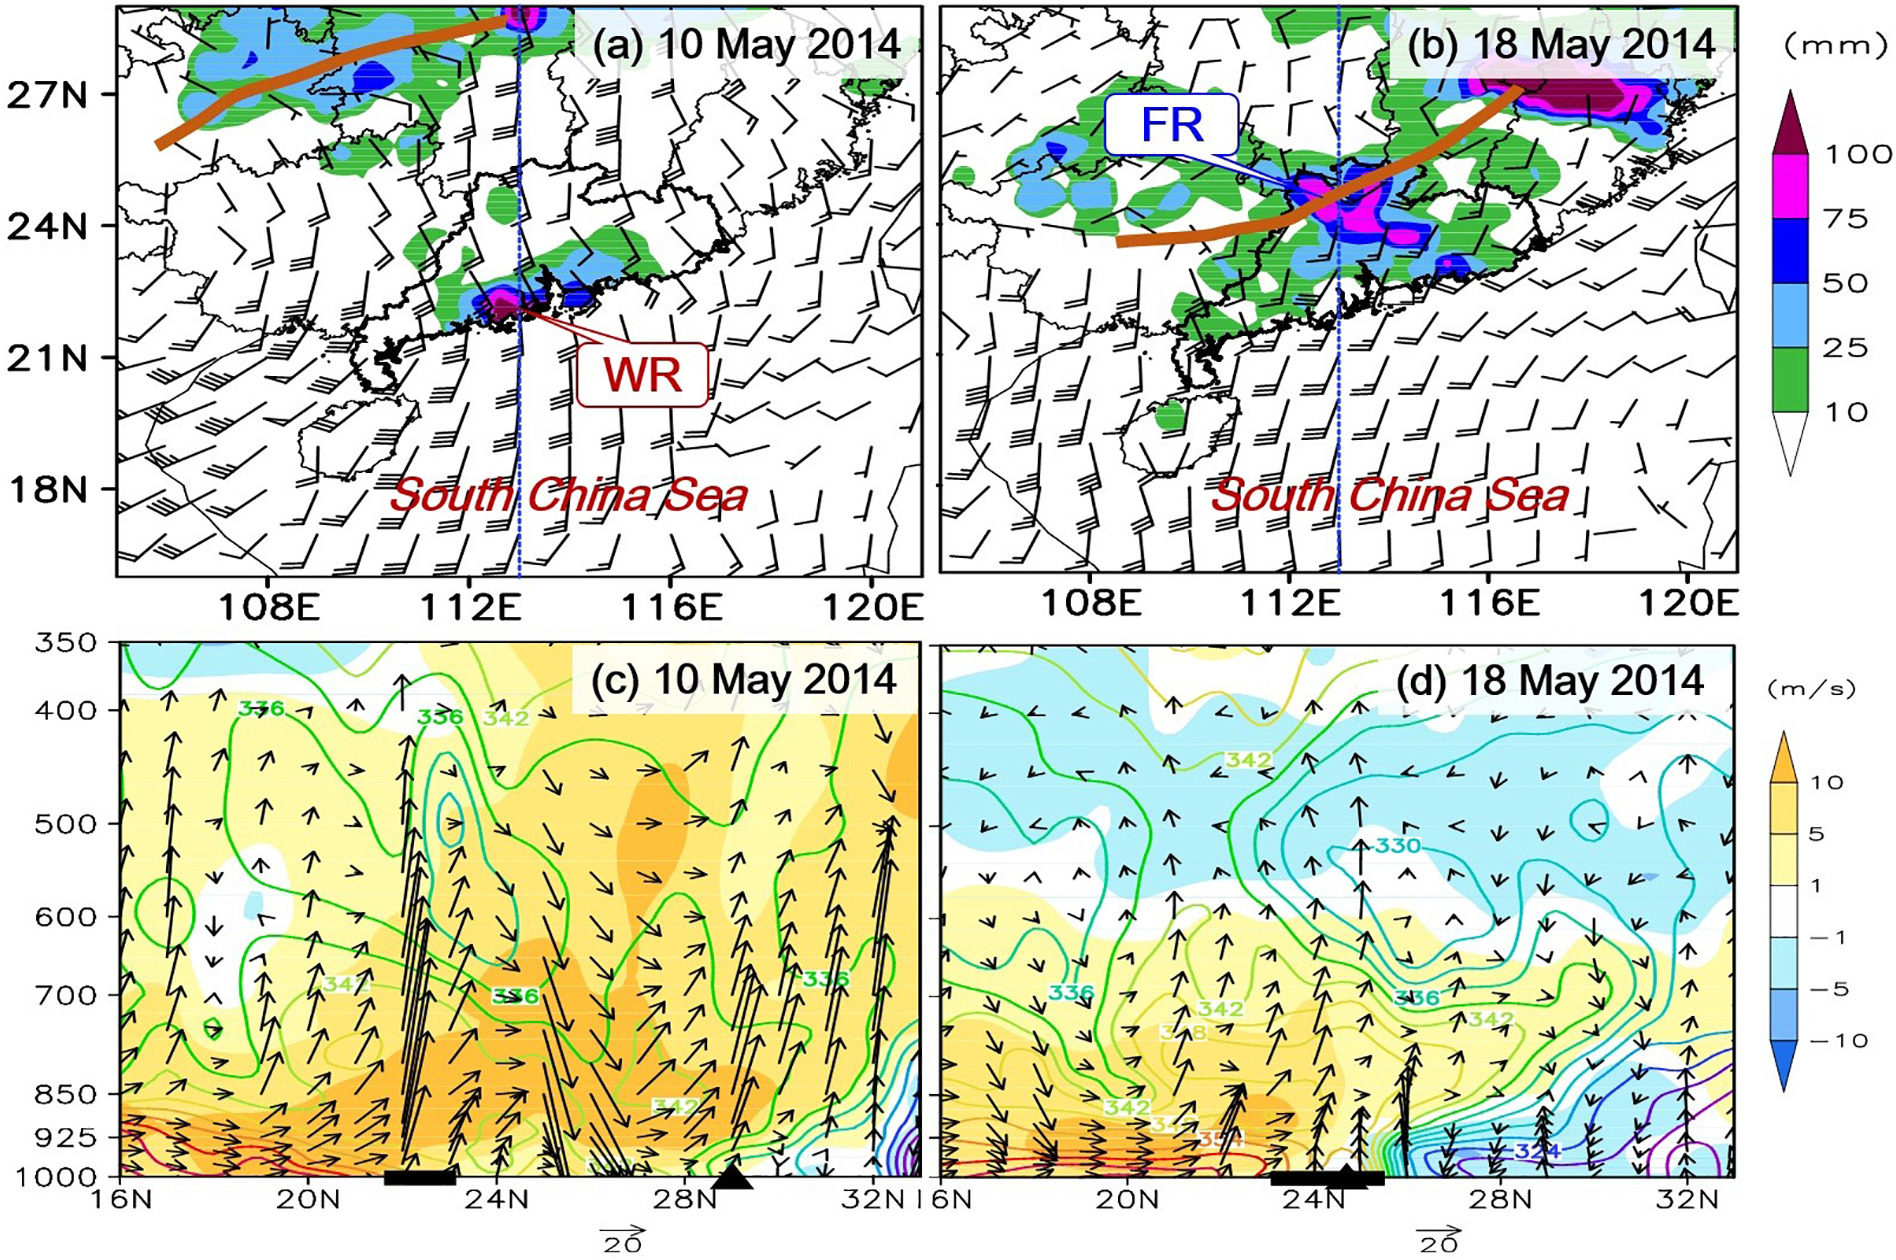
\includegraphics[width=0.6\textwidth]{1-s2.0-S0169809519302285-gr1.jpg}
	\caption{Distributions of precipitation and the circulation situation at (a, c) 0800 LST on 10 May 2014 and (b, d) 0800 LST on 18 May 2014: (a, b) 925-hPa wind field (each bar represents 4 m/s) and cumulative precipitation in the past 24 h (shaded, mm); (c, d) vertical circulation along 113°E, meridional wind (shaded, m/s) and potential pseudo-equivalent temperature (contoured every 3 K). The solid brown lines and dotted blue lines in (a, b) identify the positions of the shear lines and 113°E, respectively. The solid squares and triangles in (c, d) are the latitudinal position of the precipitation areas and the fronts, respectively.}
    \label{fig:1}
\end{figure}

\section{结论与展望}
\input{chapters/Perspectives.tex}

\acknowledgement
首先特别感谢iamty制作的thesis-NJFU南京林业大学模板为本项目提供了宝贵的借鉴和参考,
同时Qsion在NJAU-Thesis项目中提供了历年理工科模板使我们在本次重制过程中少走了许多弯路。

此外,本项目学习了上海交通大学SJTUThesis,中国科学技术大学ustcthesis操作中使用的宏包拓展。

再次对诸多优秀的开源模板的贡献者表示衷心的感谢!

\thesisreferences
\end{document}